\stepcounter{tableCounter} % Increment counter
\setcounter{rowCounter}{0} % Reset counter
\begin{tabularx}{\textwidth}{|>{\columncolor{tableColumnColor}}c|>{\columncolor{tableColumnColor}}c|>{\hsize=1.2\hsize}X|>{\hsize=.8\hsize}X|}
  \hline
  \rowcolor{tableHeaderColor}
  ID & Check & Description & Comments \\ \hline

  \multicolumn{4}{|c|}{\cellcolor{tableColumnColor} \textit{To be performed at least 3 days prior to the Briefing}} \\ \hline
  
  \cellcolor{cyan}
  \procedureItem{Write down starting time}{Start time: }
  
  \cellcolor{cyan}
  \procedureItem{Define test name (header)}{}
  
  \cellcolor{cyan}
  \procedureItem{Define test description (sec. A)}{}
  
  \cellcolor{cyan}
  \procedureItem{Define who will attend the test (sec B.)}{}
  
  \cellcolor{cyan}
  \procedureItem{Define test parameters (sec. C)}{}
  
  \cellcolor{cyan}
  \procedureItem{Coordinate testing time slots with airfield responsible (Julius Wymann), e.g.: 
    \begin{itemize}
      \item Wednesday, 19.04.2023: Cryogenic Filling \& CF
      \item Thursday, 20.04.2023: Buffer
      \item Friday, 21.04.2023: Preparations for Firing
      \item Saturday, 22.04.2023: Firing
    \end{itemize}}{}
  
  \cellcolor{cyan}
  \procedureItem{Coordinate testing time slots with supervisors (i.e., set up a when2meet, ideally 1 week prior to the test)}{}
  
  \cellcolor{cyan}
  \procedureItem{Organize gas and gas transport if needed}{}
  \multicolumn{4}{|c|}{\cellcolor{tableColumnColor} \textit{To be performed at least 6 working hours prior to the Briefing}} \\ \hline
  \cellcolor{cyan}
  \procedureItem{Check weather forecast according to Meteo Swiss: 
    \begin{itemize}
      \item Temperatures within operating temperatures (0$^\circ$C -- 35$^\circ$C)
      \item Limited wind, no hard rain and no storms (DACS must stay dry)
    \end{itemize}}{}
  
  \cellcolor{cyan}
  \procedureItem{Check that testing area (airfield) is unoccupied (e.g., no tents, trucks, airplanes, \dots)}{}
  
  \cellcolor{cyan}    
  \procedureItem{Define starting time of the test}{}
  
  \cellcolor{cyan}    
  \procedureItem{Define timeplan:
    As per 2nd Water Cold Flow:
    \begin{itemize}
      \item H-6h00min: Printing Procedures
      \item H-3h00min: Pre-Preparations
      \item H-2h00min: Packing
      \item H-0h15min: Meeting of all people at Hangar
      \item H-0h00min: Briefing
      \item H+0h15min: Transfer to Airfield
      \item H+0h45min: Installation
      \item H+1h25min: Preconditions Check
      \item H+1h35min: Pre-Firing Checks
      \item H+2h35min: Filling
      \item H+3h20min: 10min Break
      \item H+3h30min: System Activation
      \item H+3h50min: 1st Cold Flow
      \item H+4h15min: 2nd Cold Flow
      \item H+4h20min: Safe State Establishment
      \item H+5h15min: Deinstallation
      \item H+5h35min: Packing
      \item H+5h45min: Return to IPZ
      \item H+6h00min: Debriefing
    \end{itemize}}{}
  
  \cellcolor{cyan}    
  \procedureItem{Inform all attendees about:
  \begin{itemize}
    \item Date and Location
    \item Scope (Short Test Description)
    \item Timeline (See 1.12.)
    \item Attendees
    \item Safety (Operation Safety Concept, Emergency Contact List)
    \item Organizational Stuff (Bring your ID's, Weather Conditions, Bring something to eat, Proper clothing for working with LOX)
  \end{itemize}}{}
  
  \cellcolor{cyan}    
  \procedureItem{Check that access request to airfield for all attendees has been sent out to MP (check on excel list)}{}
  
  \cellcolor{cyan}    
  \procedureItem{Check that emergency responsibles in the \textit{\underline{Contingency Procedures}} are filled out}{}
  
  \cellcolor{cyan}    
  \procedureItem{Check that Emergency Driver 1 and Emergency Driver 2 are NEVER working on the pressurized system at the same time (no two of TC, SO and PSS1)}{}
  
  \cellcolor{cyan}    
  \procedureItem{Check that \textit{\underline{Firing Organization Chart}} is up-to-date}{}
  
  \cellcolor{cyan}    
  \procedureItem{Print out all relevant procedures (sec. D)}{}
  
  \cellcolor{cyan}    
  \procedureItem{Charge all walkie-talkies}{}
  
  \cellcolor{cyan}    
  \procedureItem{Charge GoPros and further cameras}{}
  
  \cellcolor{cyan}    
  \procedureItem{Charge mobile phone if necessary (ensure a charger cable is available)}{}
  
  \cellcolor{green}    
  \procedureItem{Charge mobile phone if necessary (ensure a charger cable is available)}{}
  
  \cellcolor{yellow}
  \procedureItem{Update config file and csv files on Sharepoint under 08\_DACS\_01\_Software\_07\_Configuration:
    \begin{itemize}
      \item Update firing parameter specification
      \item Choose sequence and update activation times
      \item Update sensor thresholds
      \item Mark all changes pink
    \end{itemize}}{}
  \multicolumn{4}{|c|}{\cellcolor{tableColumnColor} \textit{To be performed 30 min before the Briefing}} \\ \hline
  
  \cellcolor{cyan}
  \procedureItem{Re-Check weather forecast according to Meteo Swiss:
    \begin{itemize}
      \item Temperatures within operating temperatures (0$^\circ$C -- 35$^\circ$C)
      \item Limited wind, no hard rain and no storms (DACS must stay dry)
    \end{itemize}}{}
  
  \cellcolor{cyan}    
  \procedureItem{Fill out environmental conditions (sec. E)}{}
  
  \cellcolor{green}    
  \procedureItem{Evaluate risk in case of adverse weather conditions (heavy rain, \dots)}{}
  
  \cellcolor{cyan}    
  \procedureItem{Check that all relevant procedures are printed out (sec. D)}{}
  
  \cellcolor{green}    
  \procedureItem{Check that all attendees have read the \textit{\underline{Operation Safety Concept}}}{}
  \cellcolor{green}   
  \procedureItem{Check that all attendees have signed the \textit{\underline{Safety Signatures}}}{}
  
  \cellcolor{green}    
  \procedureItem{Check that all attendees have filled out the \textit{\underline{Emergency Contact List}}}{}
  
  \cellcolor{green}    
  \procedureItem{Head to MP to get access badges and keys:
    \begin{itemize}
      \item Bring little bag (if many badges)
      \item Key to Hunter-Stübli: ``\textbf{2.16 Pisten-Baracke}''
      \item Key for Gate: ``\textbf{19.3 Zauntor Halle 1}''
    \end{itemize}
    Do not ask for ``19.22'' !!
  }{Picture of the keys:
    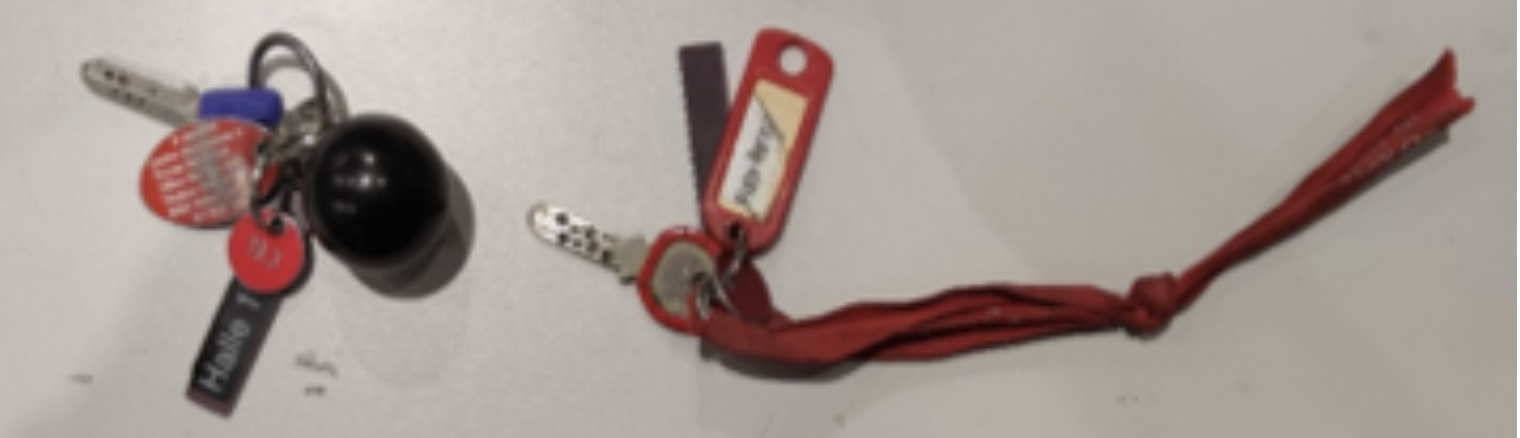
\includegraphics[width=\textwidth]{assets/picture-keys.png}
  }
  
  \cellcolor{cyan}    
  \procedureItem{Re-Check that testing area (airfield) is unoccupied (e.g., no tents, trucks, airplanes, \dots)}{}
  
  \cellcolor{cyan}    
  \procedureItem{Get final clearance to enter airfield:
    \begin{itemize}
      \item If wind vane still up, flight operations are still ongoing
      \item If wind vane is down, limited flight operations are still possible
    \end{itemize}
    Call PiWa if suspected flight operations or earlier entry desired. Installation during flight operations is generally possible depending on the circumstances.
    
    Contacts:
    \begin{itemize}
      \item Pistenwagen (PiWa): 079 829 12 18 (Martin Larcher oder Durchdiener)
      \item Roger Gisler (C Support Flugbetrieb): 058 481 79 18 / 079 944 42 52
    \end{itemize}}{}
  
  \cellcolor{cyan}    
  \procedureItem{$\rightarrow$ Ready for \textbf{Briefing}}{}
\end{tabularx}